\documentclass{eplDoc}
\usepackage{placeins}


\newcommand{\docType}	{Assignment 1 : Corpus Processing}
\newcommand{\docDate}	{01/03/2012}
\newcommand{\docAuthor}	{gr10 : Mulders Corentin, Pelsser François}
\newcommand{\courseCode}{LINGI2263}
\newcommand{\courseName}{Computational linguistics}
\usepackage{syntax}
\begin{document}
\maketitle
\newpage

\section{Global acrhitecture}

\subsection{Program architecture}

Our program is composed of three parts. The first and main part is a set of unitex graphs that are used to single out the desired data with tags. The second part is a python script that applies these graphs to the files to get tagged files. The last one is a other python script that parses the tagged files to create a cleaned up results file. 

\subsection{Use of Unitex tools}

We use unitex to perform the patterns matchings that allow us to find the informations in the text. What we did is that for each desired information (such as gender, age, height,...) we created a unitex graph file. This graph can be used to ad tags around the wanted values. For example the age graph would surround all occurrences of a patients age with \{age\} and \{/age\} in the text file. \\ 
Some of these graphs are very basic like the gender graph that simply looks for occurrences of "male" or "female". Others are more complex like the height graph that needs to be able to transform a height in the form "5 feet 3 inches" to "5'3"" for example, as well as specify in the tag what the unit used is so that our python script can convert it later. \\ 

\section{Extraction patterns}

\subsection{Context and other idiosyncrasies used in solution}

We relied on different idiosyncrasies to single out the informations depending of what we were looking for. Here is a brief explanation of how we extracted data for each type of information: 

\subsubsection{gender}
We simply looked for the "male" or "female" word. Most of the time if one of these words appears in a medical report it was to describe the patient's gender. 

\subsubsection{age}

We looked for numbers followed by the following keywords : -year-old, years old, y/o.

\subsubsection{weight}

We looked for some words (weight, weights, weight at discharge) followed by either is, of, :, =,... followed by any number followed by a weight unit. The tag used depends on the unit found. 

\subsubsection{height}

We looked for the height words followed by either is, of, :, =,... followed by any notation for a height found in the files (x cm, x m, x'y", x feet y inches,...) if the height is in feet and with a textual representation we convert it to a x'y" notation using variable sin the unitex graph. \\ 
The graph used to put tags around the values of the heights of the patients can be seen in Figure \ref{gr} as an example to show how we used variables to change the notation.
\FloatBarrier
\begin{figure}%
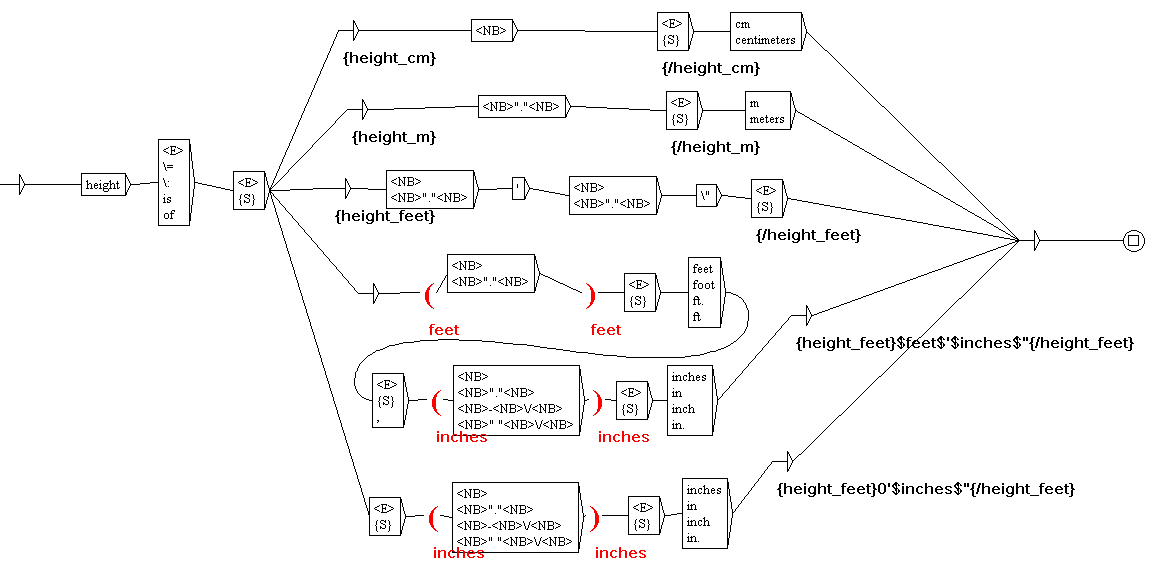
\includegraphics[width=\columnwidth]{heightgraph.png}%
\caption{Set height tags}%
\label{gr}%
\end{figure}
\FloatBarrier
\subsubsection{body mass index}

We looked for "bmi" or "body mass index" and used the value following. 

\subsubsection{Temperature}

We looked for temperature or temp keywords and detected the unit by looking for degrees celsius or C, we determined that by default the temperature was in fahrenheit if it isn't specified. 

\subsubsection{Pulse}

We looked for the "pulse" and "heart rate" keywords. 

\subsubsection{Breathing frequency}

We looked for "respiratory rate" and "RR" keywords. 

\subsubsection{Blood pressure}

We looked for the "blood pressure", "diastolic pressure", "systolic pressure" keywords. We also detect the cases where the blood pressure is expressed as a range from diastolic pressure to systolic pressure by looking for the "from...to" keywords or a simpler expression "diastolic pressure/systolic pressure". \\ 


\subsubsection{Oxygen saturation}

We looked for the "oxygen" and "O2" keywords in association with "saturation". 



\subsection{Advantages and shortcomings of our designs choices}
\subsubsection{Advantages}
\begin{itemize}
	\item Our rules are quite flexible and would work even with files with slight differences.
	\item We can extract the height of patients even though there are some very different ways to express it.
\end{itemize}
\subsubsection{Shortcomings}
\begin{itemize}
	\item We weren't able to find the conditions for the oxygen saturation measure. 
	\item We were not able to extract some informations for patients when it is expressed as a variation to a "normal" value. For example if a patient was said to have a slightly higher than average blood pressure we wouldn't get this information. 
\end{itemize}



%\subsection{Possible ways to improve results}

%We made rules that only considered one appearance of any information at a time. If a given information appears more than one time with a different %value we simply chose the last one by using the hypothesis that the medical reports are redacted chronologically. We might have used broader patterns 

\end{document}
